\section{Quantum Computing Foundations}
\noindent Before delving into quantum algorithms, it would be worthwhile to take a quick glance into the basics of quantum computing. Quantum computing uses the quantum state of a particle as the building block of information. Each such particle is called a qubit. These qubits follow the postulates of quantum mechanics\cite{shankar}, namely
\begin{enumerate}
\item The state of the particle is represented as a vector $\ket{\psi(t)}$ in a Hilbert Space.
\item The independent variables $x$ and $p$ of classical mechanics are represented by Hermitian operators $X$ and $P$ satisfying $\braketop{x}{X}{x\prime}=x\delta(x-x\prime)$ and $\braketop{x}{P}{x\prime}=-\iota\hbar\delta\prime(x-x\prime)$.
\item If a particle is in a state $\ket{\psi}$, measurement of the variable corresponding to the operator $\Omega$ will yield one of the eigenvalues $\omega$ with probability $P(\omega)\propto\left\lvert\braket{\omega}{\psi}\right\rvert ^2$. The state of the system will change from $\ket{\psi}$ to $\ket{\omega}$ as a result of the measurement.
\item The state vector $\ket{\psi}$ obeys the Schrödinger Equation $\iota\hbar\bfrac{d}{dt}\ket{\psi(t)}=\hat{H}\ket{\psi(t)}$, where $\hat{H}$ is the quantum Hamiltonian operator.
\end{enumerate}
\subsection{Qubits}
As discussed before, qubits are the particles whose quantum states store the necessary information. To retrieve the information, we perform measurements using an unitary operator that has $2$ eigenstates. These eigenstates are denoted as $\ket{0}$ and $\ket{1}$. Since the measurement operator is unitary, these eigenstates are orthonormal. The $2$ eigenstates represents the two possible values of a classical bit, except that quantum mechanics allows \textbf{superposition} and \textbf{entanglement}, which are discussed subsequently.
\subsection{Superposition}
In general, quantum mechanics is probabilistic and not deterministic, i.e., the two eigenstates may not be the only possible states of a qubit. A qubit can be in a superposition of two states, in the form $\ket{\psi}=\bfrac{\alpha\ket{0}+\beta\ket{1}}{\sqrt{2}}$ with the only requirement that $\abs{\alpha}^2+\abs{\beta}^2=1$ (this is called normalization. When a measurement is performed on this state, the state collapses to either $\ket{0}$ with probability $\abs{\alpha}^2$ or to $\ket{1}$ with probability $\abs{\beta}^2$.\\
Since $\ket{0}$ and $\ket{1}$ are orthonormal, they form an orthonormal basis for the states. Each state can then be represented in the form of a vector as
\begin{equation}
\label{eq:4.1}
\ket{\psi}=\bfrac{\alpha\ket{0}+\beta\ket{1}}{\sqrt{2}}=
\begin{pmatrix}
\alpha\\
\beta
\end{pmatrix}
\end{equation}
This immediately yields
\begin{equation*}
\ket{0}=
\begin{pmatrix}
1\\
0
\end{pmatrix}\quad
\ket{1}=
\begin{pmatrix}
0\\
1
\end{pmatrix}
\end{equation*}
Any state can now be written as the linear combination of these two states. Upon measurement, however, the superposition is lost and the system collapses to either of the eigenstates.\\
Since an operator operates on one state to produce another state, they can be viewed as transforming one vector to another. Thus, they can be expressed as matrices. The postulates of quantum mechanics dictate that these operators must be unitary to yield compatible, real-valued measurement.
\subsection{Multiple Qubits}
Often we encounter multiple qubit systems. The state of such a system is decided by the states of the individual qubits. The direct product of the basis states form the basis (also called pure states) for the multi-qubit system.\\
As an example, consider the $2$-qubit system. The basis set for such a system will be formed by the $4$ basis states : $\ket{0}\otimes\ket{0}$, $\ket{0}\otimes\ket{1}$, $\ket{1}\otimes\ket{0}$ and $\ket{1}\otimes\ket{1}$. These are notationally written as \\
\begin{equation*}
\begin{split}
\ket{00}&=
\begin{pmatrix}
1\\
0
\end{pmatrix}
\otimes
\begin{pmatrix}
1\\
0
\end{pmatrix}=
\begin{pmatrix}
1\\
0\\
0\\
0
\end{pmatrix}
\\
\ket{01}&=
\begin{pmatrix}
1\\
0
\end{pmatrix}
\otimes
\begin{pmatrix}
0\\
1
\end{pmatrix}=
\begin{pmatrix}
0\\
1\\
0\\
0
\end{pmatrix}
\end{split}
\end{equation*}
\begin{equation*}
\begin{split}
\ket{10}&=
\begin{pmatrix}
0\\
1
\end{pmatrix}
\otimes
\begin{pmatrix}
1\\
0
\end{pmatrix}=
\begin{pmatrix}
0\\
0\\
1\\
0
\end{pmatrix}
\\
\ket{11}&=
\begin{pmatrix}
0\\
1
\end{pmatrix}
\otimes
\begin{pmatrix}
0\\
1
\end{pmatrix}=
\begin{pmatrix}
0\\
0\\
0\\
1
\end{pmatrix}
\end{split}
\end{equation*}

Any two-qubit system is a superposition of the $4$ states mentioned above. However, not all two-qubit states are expressible as a direct product of two one-qubit states. This is called \textbf{entanglement}, which forms the basis for quantum teleportation, and spooky action at a distance.\\
For a multi-qubit system, we often use the decimal equivalent of a binary number to express the basis. For example, in a 4-qubit system, $\ket{12}=\ket{1100}=\ket{1}\otimes\ket{1}\otimes\ket{0}\otimes\ket{0}$.

\subsection{Quantum Gates}
Any logical circuit requires the use of gates. A classical circuit uses AND, NOT, OR etc. as gates. Likewise, a quantum circuit uses unitary operators as gates. A gate can be expressed as a matrix. Some of the useful gates are presented below.

\subsubsection*{Hadamard Gate}
The Hadamard gate is a \textbf{one-qubit} gate that is denoted by $H$. It performs the operation of transforming the standard basis of $\ket{0}$ and $\ket{1}$ into the Hadamard basis of $\ket{+}$ and $\ket{-}$ respectively as follows.
\begin{equation*}
\begin{split}
H\ket{0}&=\ket{+}=\bfrac{\ket{0}+\ket{1}}{\sqrt{2}}=
\bfrac{1}{\sqrt{2}}
\begin{pmatrix}
1\\
1
\end{pmatrix}\\
H\ket{1}&=\ket{-}=\bfrac{\ket{0}-\ket{1}}{\sqrt{2}}=
\bfrac{1}{\sqrt{2}}
\begin{pmatrix}
1\\
-1
\end{pmatrix}\\
\end{split}
\end{equation*}
The matrix representation is
\begin{equation*}
H=
\begin{pmatrix}
1&1\\
1&-1
\end{pmatrix}
\end{equation*}
The corresponding circuit diagram is given in figure \ref{Fig:4.1}
\begin{figure}[!htb]
   \begin{minipage}{\textwidth}
     \centering
     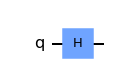
\includegraphics[scale=1]{fig04.01.png}
     \caption{Hadamard gate}
     \label{Fig:4.1}
   \end{minipage}
\end{figure}



\subsubsection*{X Gate}
The Pauli-$X$ gate is a \textbf{one-qubit} gate that is denoted by $X$ (See \ref{appB} for more details about Pauli Gates). It performs the operation of a classical NOT, i.e., it operates like the Pauli matrix $\sigma_x$ as follows. 
\begin{equation*}
\begin{split}
X\ket{0}&=\ket{1}=
\begin{pmatrix}
0\\
1
\end{pmatrix}\\
X\ket{1}&=\ket{0}=
\begin{pmatrix}
1\\
0
\end{pmatrix}\\
\end{split}
\end{equation*}
The matrix representation is
\begin{equation*}
X=
\begin{pmatrix}
0&1\\
1&0
\end{pmatrix}
\end{equation*}
The corresponding circuit diagram is given in figure \ref{Fig:4.2}
\begin{figure}[!htb]
   \begin{minipage}{\textwidth}
     \centering
     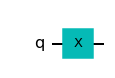
\includegraphics[scale=1]{fig04.02.png}
     \caption{$X$ gate}
     \label{Fig:4.2}
   \end{minipage}
\end{figure}

\subsubsection*{Y Gate}
The Pauli-$Y$ gate is a \textbf{one-qubit} gate that is denoted by $Y$. It operates like the Pauli matrix $\sigma_y$ as follows.
\begin{equation*}
\begin{split}
Y\ket{0}&=-\iota\ket{1}=
\begin{pmatrix}
0\\
-\iota
\end{pmatrix}\\
Y\ket{1}&=\iota\ket{0}=
\begin{pmatrix}
\iota\\
0
\end{pmatrix}\\
\end{split}
\end{equation*}
The matrix representation is
\begin{equation*}
Y=
\begin{pmatrix}
0&-\iota\\
\iota&0
\end{pmatrix}
\end{equation*}
The corresponding circuit diagram is given in figure \ref{Fig:4.3}
\begin{figure}[!htb]
   \begin{minipage}{\textwidth}
     \centering
     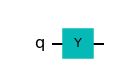
\includegraphics[scale=1]{fig04.03.png}
     \caption{$Y$ gate}
     \label{Fig:4.3}
   \end{minipage}
\end{figure}

\subsubsection*{Z Gate}
The Pauli-$Z$ gate is a \textbf{one-qubit} gate that is denoted by $Z$. It operates like the Pauli matrix $\sigma_z$ as follows.
\begin{equation*}
\begin{split}
Z\ket{0}&=\ket{0}=
\begin{pmatrix}
1\\
0
\end{pmatrix}\\
Z\ket{1}&=-\ket{1}=
-\begin{pmatrix}
0\\
1
\end{pmatrix}\\
\end{split}
\end{equation*}
The matrix representation is
\begin{equation*}
Z=
\begin{pmatrix}
1&0\\
0&-1
\end{pmatrix}
\end{equation*}
The corresponding circuit diagram is given in figure \ref{Fig:4.4}
\begin{figure}[!htb]
   \begin{minipage}{\textwidth}
     \centering
     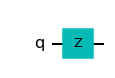
\includegraphics[scale=1]{fig04.04.png}
     \caption{$Z$ gate}
     \label{Fig:4.4}
   \end{minipage}
\end{figure}

\subsubsection*{$R_x$ Gate}
The $R_x$ gate is a \textbf{one-qubit} unitary gate that takes a parameter $\theta$. It is given by the matrix 
\begin{equation*}
R_x(\theta)=
\begin{pmatrix}
\cos\left(\bfrac{\theta}{2}\right)&-\iota \sin\left(\bfrac{\theta}{2}\right)\\
-\iota \sin\left(\bfrac{\theta}{2}\right)&\cos\left(\bfrac{\theta}{2}\right)
\end{pmatrix}
\end{equation*}

\subsubsection*{$R_y$ Gate}
The $R_y$ gate is a \textbf{one-qubit} unitary gate that takes a parameter $\theta$. It is given by the matrix 
\begin{equation*}
R_y(\theta)=
\begin{pmatrix}
\cos\left(\bfrac{\theta}{2}\right)&\sin\left(\bfrac{\theta}{2}\right)\\
\sin\left(\bfrac{\theta}{2}\right)&\cos\left(\bfrac{\theta}{2}\right)
\end{pmatrix}
\end{equation*}

\subsubsection*{$R_z$ Gate}
The $R_z$ gate is a \textbf{one-qubit} unitary gate that takes a parameter $\theta$. It is given by the matrix 
\begin{equation*}
R_z(\theta)=
\begin{pmatrix}
e^{-\iota\frac{\theta}{2}}&0\\
0&e^{\iota\frac{\theta}{2}}
\end{pmatrix}
\end{equation*}

\subsubsection*{CX Gate}
The CNOT (or CX) gate is a \textbf{two-qubit} gate that is denoted by $CX$. It operates a classical NOT, i.e., an $X$ gate on the second qubit if the first qubit is $\ket{1}$. Its working is shown below.
\begin{equation*}
\begin{split}
CX\ket{00}&=\ket{00}=
\begin{pmatrix}
1\\
0\\
0\\
0
\end{pmatrix}\\
CX\ket{01}&=\ket{01}=
\begin{pmatrix}
0\\
1\\
0\\
0
\end{pmatrix}\\
CX\ket{10}&=\ket{11}=
\begin{pmatrix}
0\\
0\\
0\\
1
\end{pmatrix}\\
CX\ket{11}&=\ket{10}=
\begin{pmatrix}
0\\
0\\
1\\
0
\end{pmatrix}\\
\end{split}
\end{equation*}
The matrix representation is
\begin{equation*}
CX=
\begin{pmatrix}
1&0&0&0\\
0&1&0&0\\
0&0&0&1\\
0&0&1&0
\end{pmatrix}
\end{equation*}
Note that the order of the qubits is important here. The corresponding circuit diagram is given in figure \ref{Fig:4.5}
\begin{figure}[!htb]
   \begin{minipage}{\textwidth}
     \centering
     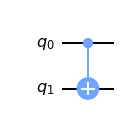
\includegraphics[scale=1]{fig04.05.png}
     \caption{$CX$ gate}
     \label{Fig:4.5}
   \end{minipage}
\end{figure}

\subsubsection*{CZ Gate}
The CZ gate is a \textbf{two-qubit} gate that is denoted by $CZ$. It is like a classical AND gate which flips the sign if and only if both qubits are $\ket{1}$. Its working is shown below.
\begin{equation*}
\begin{split}
CZ\ket{00}&=\ket{00}=
\begin{pmatrix}
1\\
0\\
0\\
0
\end{pmatrix}\\
CZ\ket{01}&=\ket{01}=
\begin{pmatrix}
0\\
1\\
0\\
0
\end{pmatrix}
\end{split}
\end{equation*}
\begin{equation*}
\begin{split}
CZ\ket{10}&=\ket{10}=
\begin{pmatrix}
0\\
0\\
1\\
0
\end{pmatrix}\\
CZ\ket{11}&=-\ket{11}=
-\begin{pmatrix}
0\\
0\\
0\\
1
\end{pmatrix}\\
\end{split}
\end{equation*}
The matrix representation is
\begin{equation*}
CZ=
\begin{pmatrix}
1&0&0&0\\
0&1&0&0\\
0&0&1&0\\
0&0&0&-1
\end{pmatrix}
\end{equation*}
Note that the order of the qubits is unimportant here. The corresponding circuit diagram is given in figure \ref{Fig:4.6}
\begin{figure}[!htb]
   \begin{minipage}{\textwidth}
     \centering
     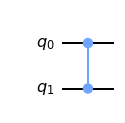
\includegraphics[scale=1]{fig04.06.png}
     \caption{$CZ$ gate}
     \label{Fig:4.6}
   \end{minipage}
\end{figure}

\subsubsection*{SWAP Gate}
The SWAP gate is a \textbf{two-qubit} gate that is denoted by $SWAP$. It swaps the two qubits. Its working is shown below.
\begin{equation*}
\begin{split}
SWAP\ket{00}&=\ket{00}=
\begin{pmatrix}
1\\
0\\
0\\
0
\end{pmatrix}\\
SWAP\ket{01}&=\ket{10}=
\begin{pmatrix}
0\\
0\\
1\\
0
\end{pmatrix}
\end{split}
\end{equation*}
\begin{equation*}
\begin{split}
SWAP\ket{10}&=\ket{01}=
\begin{pmatrix}
0\\
1\\
0\\
0
\end{pmatrix}\\
SWAP\ket{11}&=\ket{11}=
\begin{pmatrix}
0\\
0\\
0\\
1
\end{pmatrix}\\
\end{split}
\end{equation*}
The matrix representation is
\begin{equation*}
SWAP=
\begin{pmatrix}
1&0&0&0\\
0&0&1&0\\
0&1&0&0\\
0&0&0&1
\end{pmatrix}
\end{equation*}
Note that the order of the qubits is unimportant here. The corresponding circuit diagram is given in figure \ref{Fig:4.7}
\begin{figure}[!htb]
   \begin{minipage}{\textwidth}
     \centering
     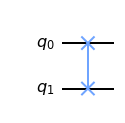
\includegraphics[scale=1]{fig04.07.png}
     \caption{$SWAP$ gate}
     \label{Fig:4.7}
   \end{minipage}
\end{figure}

\subsubsection*{MCT Gate}
The Multi Controlled Toffoli (MCT) gate is a \textbf{multi-qubit} gate that is denoted by $MCT$.It puts a negative sign on the target qubit if all the control qubits are $\ket{1}$.
The matrix representation is
\begin{equation*}
MCT=
\begin{pmatrix}
1&0&\dots&0&0\\
0&1&\dots&0&0\\
\vdots&\vdots&\ddots&\vdots&\vdots\\
0&0&\dots&1&0\\
0&0&\dots&0&-1
\end{pmatrix}
\end{equation*}
Note that the order of the qubits is unimportant here. The corresponding circuit diagram is given in figure \ref{Fig:4.8}
\begin{figure}[!htb]
   \begin{minipage}{\textwidth}
     \centering
     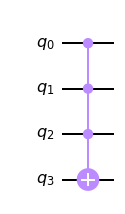
\includegraphics[scale=1]{fig04.08.png}
     \caption{$MCT$ gate on $4$ qubits}
     \label{Fig:4.8}
   \end{minipage}
\end{figure}


Note that gates can be cascaded. The order of operations of the gates is important. If we have gates $G_1$ and $G_2$, then $G_1G_2\ket{\psi}$ means $G_2$ is operated first on $\ket{\psi}$ and then $G_1$ is applied on the resulting states. Sometimes, cascading gates may result in an equivalent gate. As an example, cascading the operation of $H$ followed by $X$ is same as $R_y$ since $XH=R_y$ (this is trivial and can be easily verified). 

\subsection{Entanglement}
Entanglement is the is phenomenon where two or more quantum particles (qubits) are correlated and measurement of one particle collapses the wavefunction of the other particles. A simple example of an entangled state is
\begin{equation*}
\ket{\psi}=\bfrac{\ket{00}+\ket{11}}{\sqrt{2}}
\end{equation*}
If the measurement of the first particle collapses to $\ket{0}$, the second particle collapses to $\ket{0}$ as well.\\
Note that entangled states cannot be factored into a direct product of two single qubit states. This is a phenomenon that is purely quantum mechanical and is extremely useful in secure communication. This is because, since a measurement of any one particle collapses the wavefunction of the other particles as well, eavsdroppers will never go unnoticed, unlike in the classical case. To measure entanglement, we use the concepts of Bell's inequality. Entanglement has led to several paradoxes as well, the most famous of which is the EPR paradox presented in \ref{appC}